% TODO:














%%%%%%%%%%%%%%%%%%%%%%%%%%%%%%%%%%%%%%%%%
% Beamer Presentation
% LaTeX Template
% Version 1.0 (10/11/12)
%
% This template has been downloaded from:
% http://www.LaTeXTemplates.com
%
% License:
% CC BY-NC-SA 3.0 (http://creativecommons.org/licenses/by-nc-sa/3.0/)
%
%%%%%%%%%%%%%%%%%%%%%%%%%%%%%%%%%%%%%%%%%

%----------------------------------------------------------------------------------------
%	PACKAGES AND THEMES
%----------------------------------------------------------------------------------------

\documentclass{beamer}

\mode<presentation> {

% The Beamer class comes with a number of default slide themes
% which change the colors and layouts of slides. Below this is a list
% of all the themes, uncomment each in turn to see what they look like.

%\usetheme{default}
%\usetheme{AnnArbor}
%\usetheme{Antibes}
%\usetheme{Bergen}
%\usetheme{Berkeley}
%\usetheme{Berlin}
%\usetheme{Boadilla}
%\usetheme{CambridgeUS}
%\usetheme{Copenhagen}
%\usetheme{Darmstadt}
%\usetheme{Dresden}
%\usetheme{Frankfurt}
%\usetheme{Goettingen}
%\usetheme{Hannover}
%\usetheme{Ilmenau}
%\usetheme{JuanLesPins}
%\usetheme{Luebeck}
\usetheme{Madrid}
%\usetheme{Malmoe}
%\usetheme{Marburg}
%\usetheme{Montpellier}
%\usetheme{PaloAlto}
%\usetheme{Pittsburgh}
%\usetheme{Rochester}
%\usetheme{Singapore}
%\usetheme{Szeged}
%\usetheme{Warsaw}

% As well as themes, the Beamer class has a number of color themes
% for any slide theme. Uncomment each of these in turn to see how it
% changes the colors of your current slide theme.

%\usecolortheme{albatross}
%\usecolortheme{beaver}
%\usecolortheme{beetle}
%\usecolortheme{crane}
%\usecolortheme{dolphin}
%\usecolortheme{dove}
%\usecolortheme{fly}
%\usecolortheme{lily}
%\usecolortheme{orchid}
%\usecolortheme{rose}
%\usecolortheme{seagull}
%\usecolortheme{seahorse}
%\usecolortheme{whale}
%\usecolortheme{wolverine}

%\setbeamertemplate{footline} % To remove the footer line in all slides uncomment this line
%\setbeamertemplate{footline}[page number] % To replace the footer line in all slides with a simple slide count uncomment this line

%\setbeamertemplate{navigation symbols}{} % To remove the navigation symbols from the bottom of all slides uncomment this line
}

\usepackage[utf8]{inputenc}
\usepackage[russian]{babel}
\usepackage{cmap}

\usepackage{MnSymbol,wasysym}
\usepackage{verbatim}
\usepackage{fancybox}
\usepackage{ulem}
\usepackage{tikz}
\usetikzlibrary{positioning}
\usepackage{scalefnt}
\usetikzlibrary{arrows,shapes,positioning,shadows,trees,calc,backgrounds,fit,positioning}

\usepackage{graphicx} % Allows including images
\usepackage{booktabs} % Allows the use of \toprule, \midrule and \bottomrule in tables
\usepackage{textcomp}
\usepackage{listings}
\usepackage{color}
\usepackage{xcolor}
\usepackage{changepage}

\definecolor{mygreen}{rgb}{0,0.6,0}
\definecolor{mygray}{rgb}{0.5,0.5,0.5}
\definecolor{mymauve}{rgb}{0.58,0,0.82}

\lstset{ %
  backgroundcolor=\color{white},   % choose the background color; you must add \usepackage{color} or \usepackage{xcolor}
  basicstyle=\footnotesize,        % the size of the fonts that are used for the code
  breakatwhitespace=false,         % sets if automatic breaks should only happen at whitespace
  breaklines=true,                 % sets automatic line breaking
  captionpos=b,                    % sets the caption-position to bottom
  commentstyle=\color{mygreen},    % comment style
  deletekeywords={...},            % if you want to delete keywords from the given language
  escapeinside={\%*}{*)},          % if you want to add LaTeX within your code
  extendedchars=true,              % lets you use non-ASCII characters; for 8-bits encodings only, does not work with UTF-8
  frame=single,                    % adds a frame around the code
  keepspaces=true,                 % keeps spaces in text, useful for keeping indentation of code (possibly needs columns=flexible)
  keywordstyle=\color{blue},       % keyword style
  language=Octave,                 % the language of the code
  morekeywords={*,...},            % if you want to add more keywords to the set
  numbers=left,                    % where to put the line-numbers; possible values are (none, left, right)
  numbersep=5pt,                   % how far the line-numbers are from the code
  numberstyle=\tiny\color{mygray}, % the style that is used for the line-numbers
  rulecolor=\color{black},         % if not set, the frame-color may be changed on line-breaks within not-black text (e.g. comments (green here))
  showspaces=false,                % show spaces everywhere adding particular underscores; it overrides 'showstringspaces'
  showstringspaces=false,          % underline spaces within strings only
  showtabs=true,                  % show tabs within strings adding particular underscores
  stepnumber=1,                    % the step between two line-numbers. If it's 1, each line will be numbered
  stringstyle=\color{mymauve},     % string literal style
  tabsize=4,                       % sets default tabsize to 2 spaces
  %title=\lstname                   % show the filename of files included with \lstinputlisting; also try caption instead of title
}

\graphicspath{{./figures/}}

%----------------------------------------------------------------------------------------
%	TITLE PAGE
%----------------------------------------------------------------------------------------

\title[Обработка и исполнение запросов: лекция 3]{Обработка и исполнение запросов в СУБД (Лекция 3) \\~\\ Классические системы: гистограммы и оценка промежуточных результатов\\~\\ v6} % The short title appears at the bottom of every slide, the full title is only on the title page

\author{Георгий Чернышев} % Your name
\institute[ВШЭ] % Your institution as it will appear on the bottom of every slide, may be shorthand to save space
{
Высшая Школа Экономики \\ % Your institution for the title page
\medskip
\textit{chernishev@gmail.com} % Your email address
}
%\date{\today} % Date, can be changed to a custom date

\date{16 сентября 2020 г.}

\begin{document}

\begin{frame}
\titlepage % Print the title page as the first slide
\end{frame}

\begin{comment}
\begin{frame}
\frametitle{Overview} % Table of contents slide, comment this block out to remove it
\tableofcontents % Throughout your presentation, if you choose to use \section{} and \subsection{} commands, these will automatically be printed on this slide as an overview of your presentation
\end{frame}
\end{comment}

\begin{frame}
\frametitle{Гистограммы I}

История \cite{Ioannidis2003}:
\begin{itemize}
  \setlength\itemsep{1em}
  \item $\iota \sigma \tau os$ (istos, ``мачта'') + $\gamma \rho \alpha \mu \mu \alpha$ (gram-ma, ``надпись'');
  \item Термин придумал Karl Pearson, есть ссылки с лекции по статистике 1892 г;
  \item Много источников указывают на то, что такие объекты использовались гораздо раньше;
  \item Bar charts: ``Commercial and Political Atlas (London 1786), William Playfair'', подвид гистограмм.
\end{itemize}

\end{frame}

\begin{frame}
\frametitle{Гистограммы II}

Применение в информатике:
\begin{itemize}
  \setlength\itemsep{1em}
  \item в обработке изображений и системах компьютерного зрения;
  \item в геоинформационных системах;
  \item в базах данных: сжатие данных и аппроксимация распределений
  \begin{itemize}
    \item оценка селективности;
    \item приближенные ответы на запросы (для оптимизации);
    \item фидбек на пользовательские запросы, получаемый перед выполнением (профилирование запросов).
  \end{itemize}  
\end{itemize}

\end{frame}

% 

\begin{frame}
\frametitle{Распределение данных}

\begin{itemize}
  \setlength\itemsep{1em}
  \item Это набор пар вида (значение, частота);
  \item Знание распределения позволит оптимизировать запросы;
  \item Оно большое, если хранить всё, то выигрыша не будет :(
\end{itemize}

$\longrightarrow$ Надо \alert{дешево} аппроксимировать распределение данных.\\~\\

Для этого и используются гистограммы.

\end{frame}

\begin{frame}
\frametitle{Как оптимизировать?}

\begin{figure}[htb]
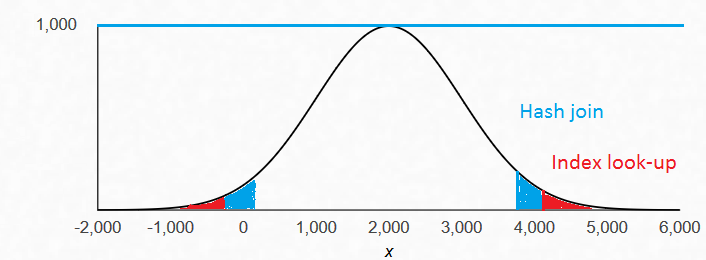
\includegraphics[width=\textwidth,height=0.39\textheight,keepaspectratio]{normal1.png} 
\end{figure}

Q1: SELECT X FROM $T_1$ WHERE X = $\alpha$;

\begin{itemize}
  \item Если выбирается мало записей~--- индекс по $T_1$, 
  \item Иначе~--- последовательный просмотр.
\end{itemize}

Q2: SELECT Z FROM $T_1$, $T_2$ WHERE $T_1$.X = $T_2$.Y AND $T_1$.X = $\alpha$;

\begin{itemize}
  \item Если выбирается мало записей~--- можно hash join по $T_1$, 
  \item Иначе~--- что-то другое.
\end{itemize}

\end{frame}

\begin{frame}
\frametitle{Гистограммы III}

Гистограмма над атрибутом $X$ строится с помощью разбиения распределения данных в $X$ на $\beta (\ge 1)$ попарно различных подмножеств (называемых ведрами) и аппроксимации частот и значений в каждом ведре единым образом.
\end{frame}

\begin{frame}
\frametitle{Данные}

\begin{figure}[htb]
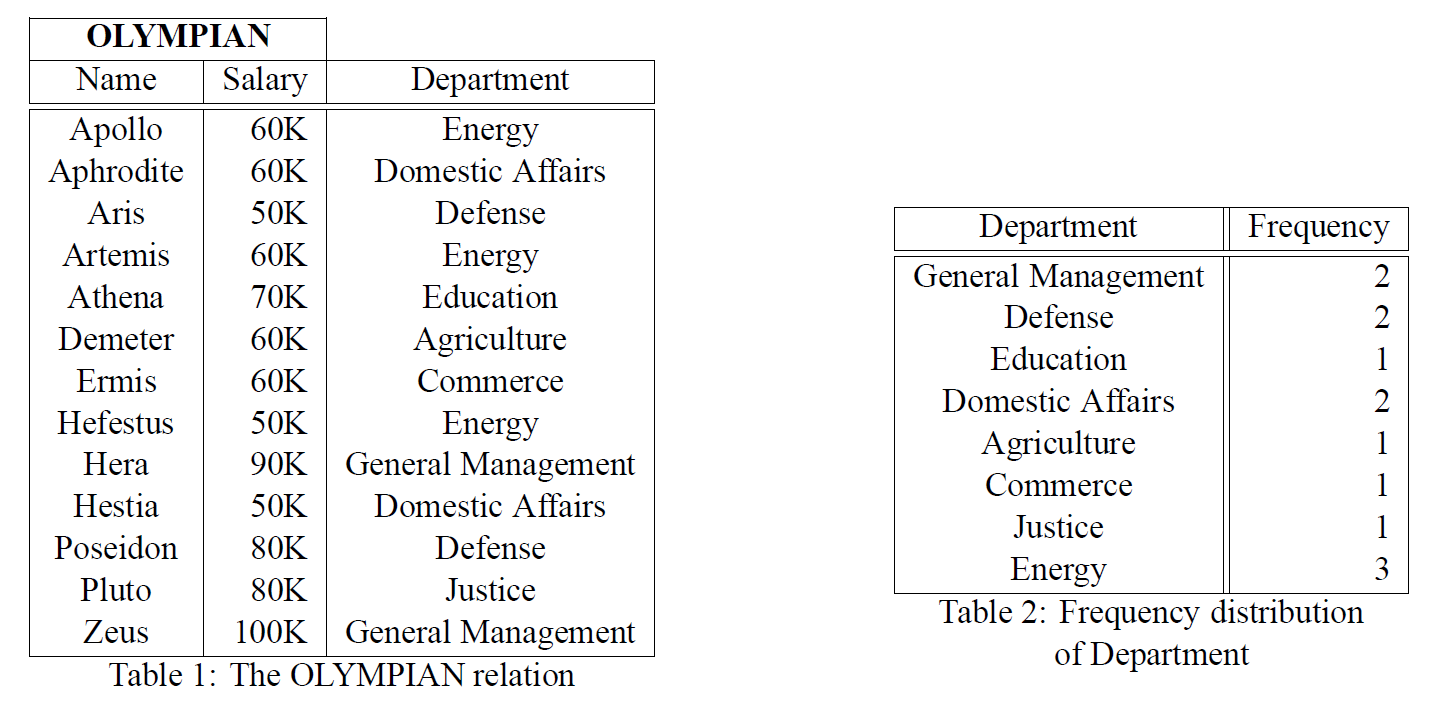
\includegraphics[width=\textwidth,height=0.79\textheight,keepaspectratio]{histogram-example-ioannidis.png} 
\footnote{\tiny{Изображение взято из \cite{Ioannidis1995}}}
\end{figure}

\end{frame}


\begin{frame}
\frametitle{Гистограммы по данным}

\begin{figure}[htb]
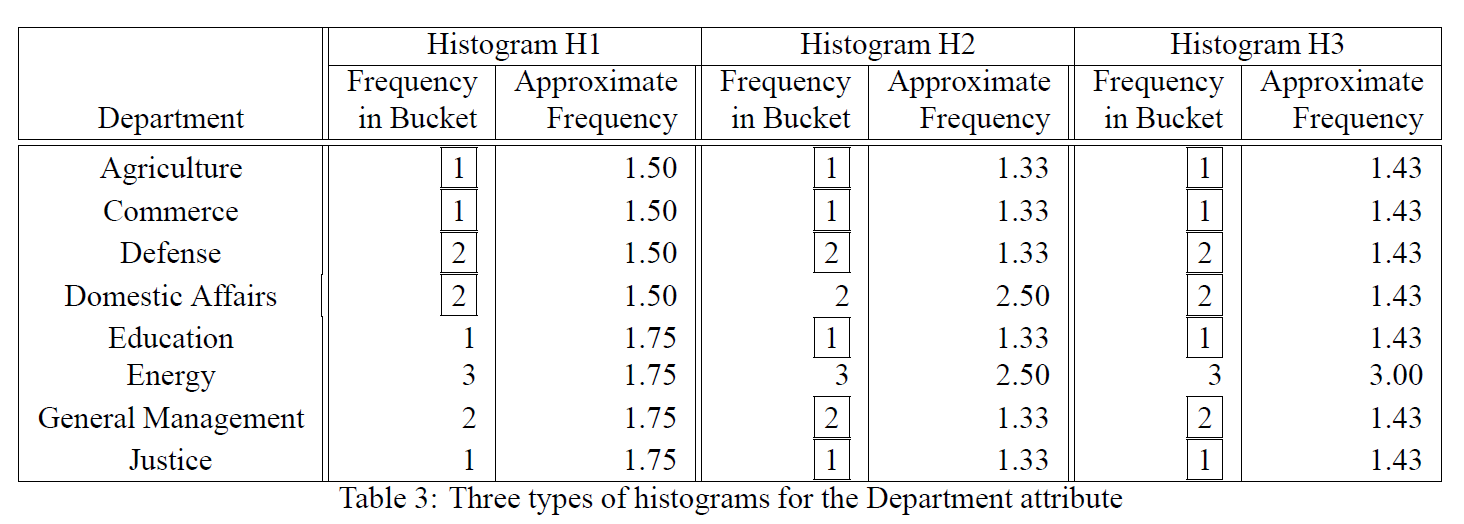
\includegraphics[width=\textwidth,height=0.79\textheight,keepaspectratio]{histogram-example-ioannidis-2.png} 
\footnote{\tiny{Изображение взято из \cite{Ioannidis1995}}}
\end{figure}

\end{frame}

\begin{frame}
\frametitle{Данные, визуально I}
\center
\begin{tikzpicture}

\draw[thick,->] (0,0) -- (9,0) node[anchor=north west] {значения};
\draw[thick,->] (0,0) -- (0,5) node[anchor=south east] {частота};
\draw[thick,-|] (0,0) -- (0,1) node[anchor=south east] {1};
\draw[thick,-|] (0,0) -- (0,2) node[anchor=south east] {2};
\draw[thick,-|] (0,0) -- (0,3) node[anchor=south east] {3};

\draw[thick,-o] (1,0) -- (1,1) node[anchor=north west] {Agriculture};
\draw[thick,-o] (2,0) -- (2,1) node[anchor=south west] {Commerce};
\draw[thick,-o] (3,0) -- (3,2) node[anchor=south west] {Defence};
\draw[thick,-o] (4,0) -- (4,2) node[anchor=north west] {Domestic Aff};
\draw[thick,-o] (5,0) -- (5,1) node[anchor=north west] {Education};
\draw[thick,-o] (6,0) -- (6,3) node[anchor=north west] {Energy};
\draw[thick,-o] (7,0) -- (7,2) node[anchor=north west] {General Mgmt};
\draw[thick,-o] (8,0) -- (8,1) node[anchor=north west] {Justice};

\end{tikzpicture}

\end{frame}


\begin{frame}
\frametitle{Гистограммы по данным, визуально I}
\center
\begin{tikzpicture}

\draw[thick,->] (0,0) -- (9,0) node[anchor=north west] {значения};
\draw[thick,->] (0,0) -- (0,5) node[anchor=south east] {частота};
\draw[thick,-|] (0,0) -- (0,1) node[anchor=south east] {1};
\draw[thick,-|] (0,0) -- (0,2) node[anchor=south east] {2};
\draw[thick,-|] (0,0) -- (0,3) node[anchor=south east] {3};

\filldraw[fill=blue!40!white, draw=black] (1,0) rectangle (4,2);
\filldraw[fill=blue!40!white, draw=black] (5,0) rectangle (8,3);

\draw[thick,-o] (1,0) -- (1,1) node[anchor=north west] {Agriculture};
\draw[thick,-o] (2,0) -- (2,1) node[anchor=south west] {Commerce};
\draw[thick,-o] (3,0) -- (3,2) node[anchor=south west] {Defence};
\draw[thick,-o] (4,0) -- (4,2) node[anchor=north west] {Domestic Aff};

\draw[thick,-o] (5,0) -- (5,1) node[anchor=north west] {Education};
\draw[thick,-o] (6,0) -- (6,3) node[anchor=north west] {Energy};
\draw[thick,-o] (7,0) -- (7,2) node[anchor=north west] {General Mgmt};
\draw[thick,-o] (8,0) -- (8,1) node[anchor=north west] {Justice};

\end{tikzpicture}

\end{frame}

\begin{frame}
\frametitle{Гистограммы по данным, визуально II}
\center
\begin{tikzpicture}

\draw[thick,->] (0,0) -- (9,0) node[anchor=north west] {значения};
\draw[thick,->] (0,0) -- (0,5) node[anchor=south east] {частота};
\draw[thick,-|] (0,0) -- (0,1) node[anchor=south east] {1};
\draw[thick,-|] (0,0) -- (0,2) node[anchor=south east] {2};
\draw[thick,-|] (0,0) -- (0,3) node[anchor=south east] {3};

\draw[dashed,-] (0,1.5)  node[anchor=south east] {1.5} -- (4,1.5);
\draw[dashed,-] (0,1.75)  node[anchor=south east] {1.75} -- (5,1.75);


\filldraw[fill=blue!40!white, draw=black] (1,0) rectangle (4,1.5);
\filldraw[fill=blue!40!white, draw=black] (5,0) rectangle (8,1.75);

\draw[thick,-o] (1,0) -- (1,1.5) node[anchor=north west] {Agriculture};
\draw[thick,-o] (2,0) -- (2,1.5) node[anchor=south west] {Commerce};
\draw[thick,-o] (3,0) -- (3,1.5) node[anchor=north west] {Defence};
\draw[thick,-o] (4,0) node[anchor=south west] {Domestic Aff} -- (4,1.5);

\draw[thick,-o] (5,0) -- (5,1.75) node[anchor=north west] {Education};
\draw[thick,-o] (6,0) node[anchor=north west] {Energy} -- (6,1.75);
\draw[thick,-o] (7,0) -- (7,1.75) node[anchor=north west] {General Mgmt};
\draw[thick,-o] (8,0) -- (8,1.75) node[anchor=south west] {Justice};

\end{tikzpicture}

\end{frame}



\begin{frame}
\frametitle{Базовые определения формально}

\begin{itemize}
  \item Отношение $R$ имеет $n$ атрибутов, обозначаемых $X_i, i \in (1, n)$;
  \item Множество значений $V_i$ атрибута $X_i$~--- значения присутствующие в $R$;
  \item Пусть $V_i = \{v_i(k): 1 \le k < D_i\}$, где $v_i(k) < v_i(j)$ когда $k < j$, тогда: 
  \begin{itemize}
    \item \alert{спред}  $s_i(k)$ для $v_i(k)$ определяется как $s_i(k) = v_i(k+1) - v_i(k)$ для $1 \le k < D_i$, при этом положим $s_i(D_i) = 1$;
    \item \alert{частота} $f_i(k)$ для $v_i(k)$ опеределяется как количество записей в $R$, у которых $X_i = v_i(k)$
    \item \alert{площадь} $a_i(k)$ определяется как $a_i(k) = f_i(k) * s_i(k)$
  \end{itemize}
  \item Распределение данных $X_i$ это множество пар $T_i = \{((v_i(1), f_i(1)), (v_i(2), f_i(2), ..., (v_i(D_i), f_i(D_i)\}$
  \item Объединенная частота $f(k_1, ..., k_n)$ комбинации значений $<v_1(k_1), ..., v_n(k_n)>$ это число записей в $R$ которые содержат $v_i(k_i)$ в атрибуте $X_i$, по всем $i$.
  \item Объединенное распределение $T_{1, ..., n}$ для $X_1, ..., X_n$ это всё множество пар (комбинация значений, объединенная частота).
\end{itemize}

\end{frame}


\begin{frame}
\frametitle{Базовые определения, визуально}
\center
\begin{tikzpicture}

\draw[thick,->] (0,0) -- (9.5,0) node[anchor=north west] {значения};
\draw[thick,->] (0,0) -- (0,5) node[anchor=south east] {частота};

\draw[thick,-o] (1,0) -- (1,4);
\draw[thick,-o] (2,0) -- (2,2);
\draw[thick,-o] (3,0) -- (3,4.5);
\draw[thick,-o] (8.5,0) -- (8.5,1);

\filldraw[fill=blue!40!white, draw=black] (4,0) rectangle (8,4) node[anchor=north east] {площадь};

\draw[thick,-o] (4,0) -- (4,4);
\draw[thick,-o] (8,0) -- (8,1.5);


\draw[thick,<->] (4,5) -- (8,5);

\node[above right=10pt of {(5,5)}, outer sep=2pt,fill=white] {спред};

\end{tikzpicture}

\end{frame}



\begin{comment}
\begin{frame}[allowframebreaks]
\frametitle{Классификация гистограмм, аспекты}

Возможных аспектов для классификации несколько, они ортогональны:

\begin{itemize}
  \item Метод фрагментирования:
  \begin{itemize}
    \item Класс фрагментирования: есть ли ограничения на ведра. Бывают: \alert{серийный класс} (serial, не пересекаются по параметру) и подкласс серийных~--- \alert{смещенных на концах} (end-biased);
    \item Параметр сортировки: некоторый параметр, значения которого для каждого элемента в распределении получаются из соответствующих значений атрибутов и частот. Пример: значение атрибута ($V$), частота ($F$), площадь ($A$);
    \item Параметр источника: некоторый параметр, отражающий наиболее важное (с точки зрения задачи оценки) свойство распределения данных. Вместе с ограничением фрагментирования однозначно определяет фрагментирование. Пример: спред (S), частота ($F$), площадь ($A$).
   
    \item Ограничение на фрагментирование: ограничение на параметр источника, уникально идентифицирующий гистограмму в классе фрагментирований. Пример: equi-sum, v-optimal, maxdiff, и compressed.
  \end{itemize}  
  \item Алгоритм создания. Часто бывает так, что для одного класса гистограмм есть несколько различных алгоритмов, с разной эффективностью.
  \item Аппроксимация значений. Каким образом значения в ведерке аппроксимируются. Обычно~--- равномерное распределение частот элементов в ведерке. 
  \item Оценка ошибки. Верхняя граница на основании информации в гистограмме.
\end{itemize}
\end{frame}
\end{comment}

\begin{frame}
\frametitle{До гистограмм}

System R:

\begin{itemize}
  \setlength\itemsep{1em}
  \item хранила минимум и максимум по каждому атрибуту;
  \item использовала предположение о равномерном распределении.
\end{itemize}

Тоже ``гистограмма'' :)\\~\\

Оценки неточны.

\end{frame}

\begin{frame}
\frametitle{Появление гистограмм в СУБД (equi-width)}

Первое появление гистограмм:
\begin{itemize}
  \setlength\itemsep{1em}
  \item Диссертация Kooi \cite{Kooi1980};
  \item Суть: множество значений разделенное на диапазоны одинаковой длины (equi-width гистограммы);
  \item Внутри ведра значения и частоты аппроксимируются исходя из: непрерывности значений + равномерного распределения частот;
  \item Встроил в СУБД Ingres, позже подхвачены и другими СУБД;
\end{itemize}

Непрерывность значений \cite{Poosala1996}: предполагаем что все значения из $V_i$ есть в указанном интервале.

\end{frame}

\begin{frame}
\frametitle{Пример: просто гистограммы}

\begin{figure}[htb]
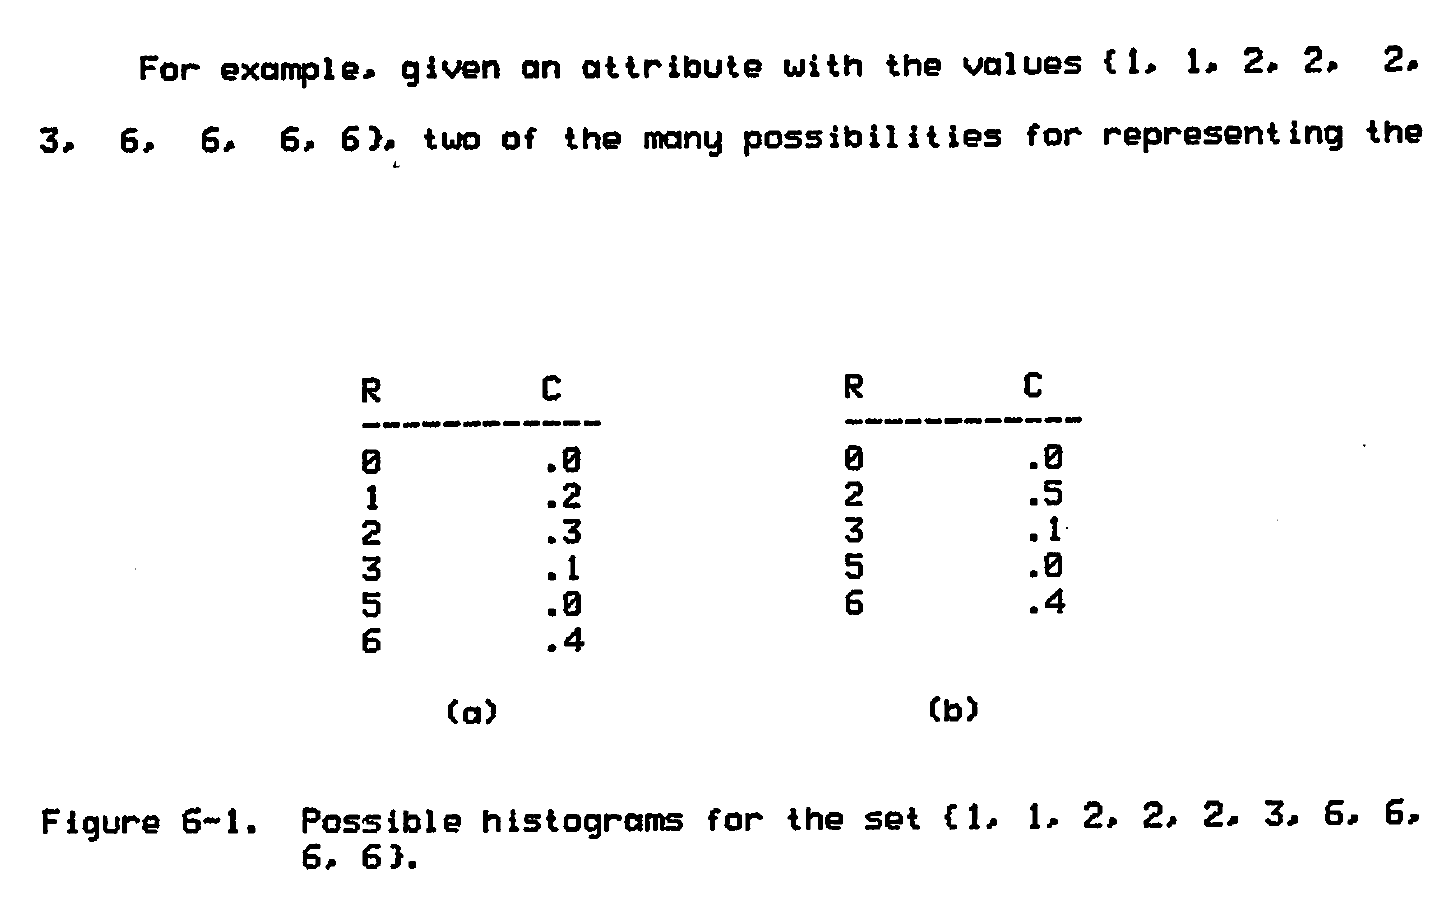
\includegraphics[width=\textwidth,height=0.79\textheight,keepaspectratio]{histogram-example-kooi.png} 
\footnote{\tiny{Изображение взято из \cite{Kooi1980}}}
\end{figure}

\end{frame}

\begin{frame}
\frametitle{Пример (6.1a), визуализация}

\begin{figure}[htb]
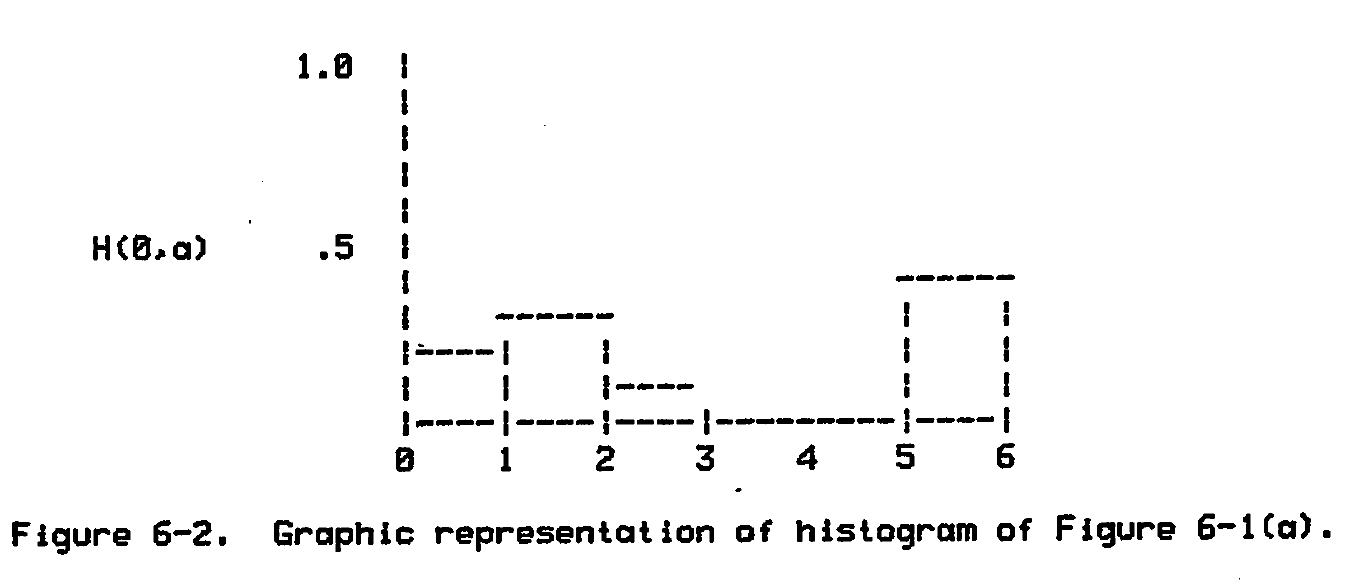
\includegraphics[width=\textwidth,height=0.79\textheight,keepaspectratio]{histogram-example-kooi-2.png} 
\footnote{\tiny{Изображение взято из \cite{Kooi1980}}}
\end{figure}

Равноширинная, если представить что есть ведра 3-4 и 4-5.

\end{frame}

\begin{frame}
\frametitle{Свойства equi-width гистограмм}


\begin{itemize}
  \item Позволяют отвечать на запросы диапазона, $x<100$;
  \begin{itemize}
    \item[] (простой проход по вёдрам)
  \end{itemize}      
  \item Плюсы: 
  \begin{itemize}
    \item сохраняют порядок;
    \item дешевы в хранении;
    \item понятно как реализовывать;
  \end{itemize}  
  \item Лучше чем подход System R;
  \item Минусы получаются из предположения о равномерности значений в ведре: 
  \begin{itemize}
    \item большой разброс;
    \item не оценить ошибку;
  \end{itemize}    
\end{itemize}

Пример\\~\\ 
данные: (1, 2000), (2, 300), (3, 100), (4, 1), (5, 1)... (10, 1)\\
гистограмма:([1-2], 1150), ([3-4], 50), ([5-6], 1), ...\\~\\
\scriptsize
А подобных распределений много и они часто встречаются в реальных данных: закон ципфа, нормальное, ...
\end{frame}

\begin{frame}
\frametitle{Первая альтернатива: equi-depth \cite{Kooi1980} \cite{Piatetsky-Shapiro1984}}

\begin{itemize}
  \setlength\itemsep{1em}
  \item Выравниваем не границы ведер, а количество записей в каждом;  
  \item Как пришли \cite{Piatetsky-Shapiro1984}: надо ограничивать высоту ведра на графике (частоту);  
  \item Тоже страдают от сложных распределений;
  \item Занимают столько же места сколько equi-width, но сложно обновлять;
  \item Тем не менее, было показано что у них лучше оценка ошибки в среднем и худшем случаях \cite{Ioannidis1995};
  \begin{itemize}
    \item[$\longrightarrow$] индустрия стала использовать их \cite{Ioannidis2003}.
  \end{itemize}      
\end{itemize}
\end{frame}

\begin{frame}
\frametitle{Схема алгоритма}

\begin{figure}[htb]
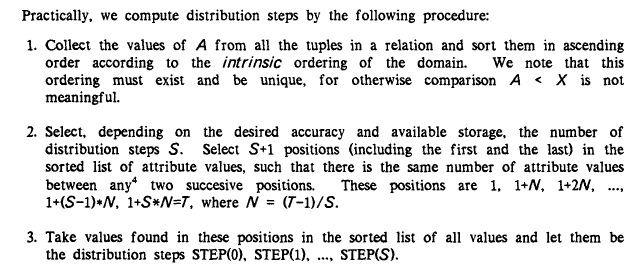
\includegraphics[width=\textwidth,height=0.79\textheight,keepaspectratio]{shapiro-algorithm.png} 
\footnote{\tiny{Изображение взято из \cite{Piatetsky-Shapiro1984}}}
\end{figure}

\end{frame}

\begin{frame}
\frametitle{Иллюстрация работы алгоритма}

\begin{figure}[htb]
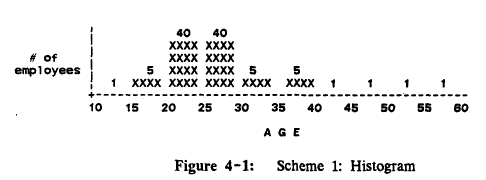
\includegraphics[width=\textwidth,height=0.35\textheight,keepaspectratio]{shapiro-1.png} 
\footnote{\tiny{Изображение взято из \cite{Piatetsky-Shapiro1984}}}
\end{figure}

\begin{figure}[htb]
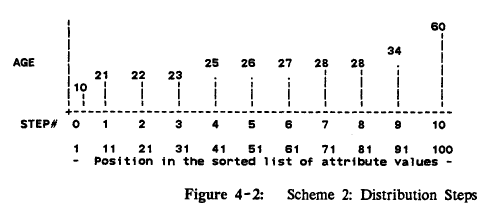
\includegraphics[width=\textwidth,height=0.36\textheight,keepaspectratio]{shapiro-2.png} 
\footnote{\tiny{Изображение взято из \cite{Piatetsky-Shapiro1984}}}
\end{figure}

\end{frame}


\begin{frame}
\frametitle{Как выполнять запросы?}

\begin{figure}[htb]
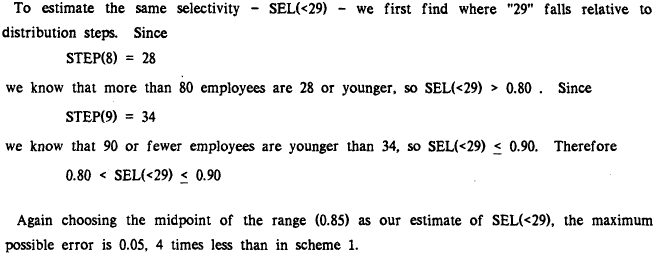
\includegraphics[width=\textwidth,height=0.65\textheight,keepaspectratio]{shapiro-3.png} 
\footnote{\tiny{Изображение взято из \cite{Piatetsky-Shapiro1984}}}
\end{figure}

\end{frame}

\begin{frame}
	\frametitle{Оффтоп: поразительный факт про сэмплинг}
	
	\begin{figure}[htb]
		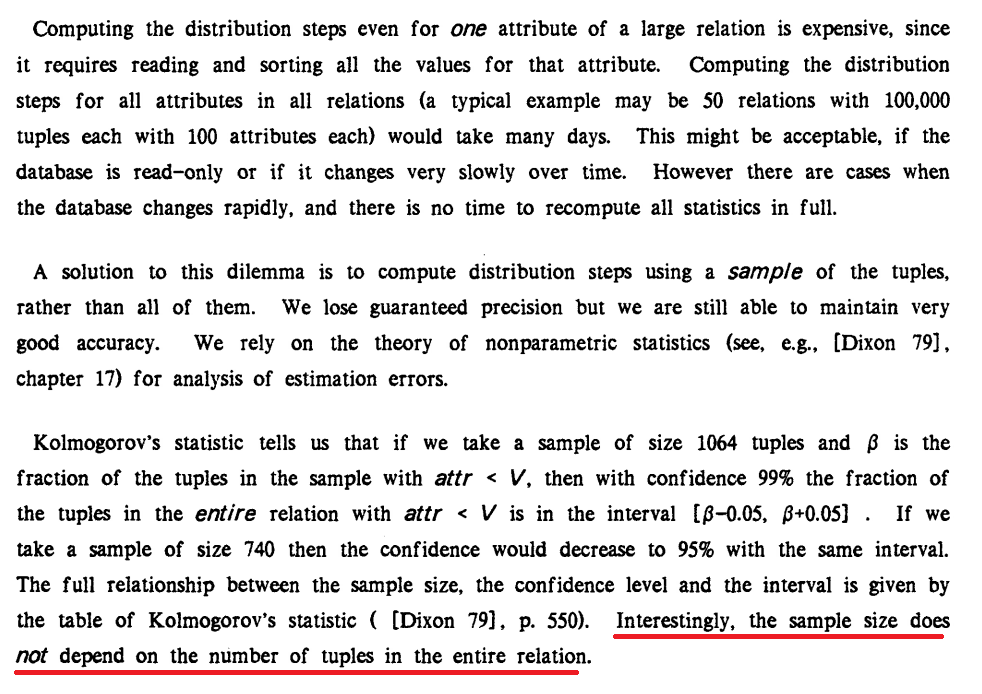
\includegraphics[width=\textwidth,height=0.75\textheight,keepaspectratio]{shapiro-4.png} 
		\footnote{\tiny{Изображение взято из \cite{Piatetsky-Shapiro1984}}}
	\end{figure}
	
\end{frame}

\begin{frame}
\frametitle{Общая схема описания гистограмм}

\scriptsize

<\alert{Ограничение на фрагментирование}> (<\alert{Параметр Сортировки}>, <\alert{Параметр Источника}>):

\begin{itemize}
	\item Класс фрагментирования (некоторые ограничения на ведра). Пример: серийный класс (serial, не пересекаются по параметру) и подкласс серийных~--- смещенных на концах (end-biased);
	\item \alert{Ограничение на фрагментирование}: ограничение на \alert{параметр источника}, уникально идентифицирующий гистограмму в классе фрагментирований. Пример: equi-sum, v-optimal, maxdiff, и compressed.	
	\item \alert{Параметр сортировки}: некоторый параметр, значения которого для каждого элемента в распределении получаются из соответствующих значений атрибутов и частот. Пример: значение атрибута ($V$), частота ($F$), площадь ($A$);
	\item \alert{Параметр источника}: некоторый параметр, отражающий наиболее важное (с точки зрения задачи оценки) свойство распределения данных. Вместе с ограничением фрагментирования однозначно определяет фрагментирование. Пример: спред ($S$), частота ($F$), площадь ($A$).	
\end{itemize}

Примеры: Equi-sum(V,S), Equi-sum(V,F), V-optimal (F,F) ...

\end{frame}


\begin{frame}
\frametitle{Применение классификации}

<\alert{Ограничение на фрагментирование}> (<\alert{Параметр Сортировки}>, <\alert{Параметр Источника}>)

\begin{itemize}
	
\item Равноширинные: серийный класс, \alert{equi-sum(V, S)}, ограничение на фрагментирование = значения исходного параметра (спреды) у каждого ведра  одинаковы.

\item Равноглубинные: серийный класс, \alert{equi-sum(V, F)}, ограничение на фрагментирование = количество элементов в ведре одинаково.

\end{itemize}

\end{frame}

\begin{frame}
\frametitle{Классификация-1}

\begin{figure}[htb]
	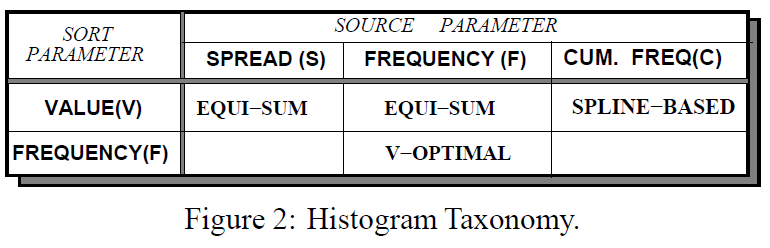
\includegraphics[width=\textwidth,height=0.65\textheight,keepaspectratio]{taxonomy-1.png} 
	\footnote{\tiny{Изображение взято из \cite{Poosala1996}}}
\end{figure}

\end{frame}



\begin{frame}
\frametitle{Серийные гистограммы}

\begin{figure}[htb]
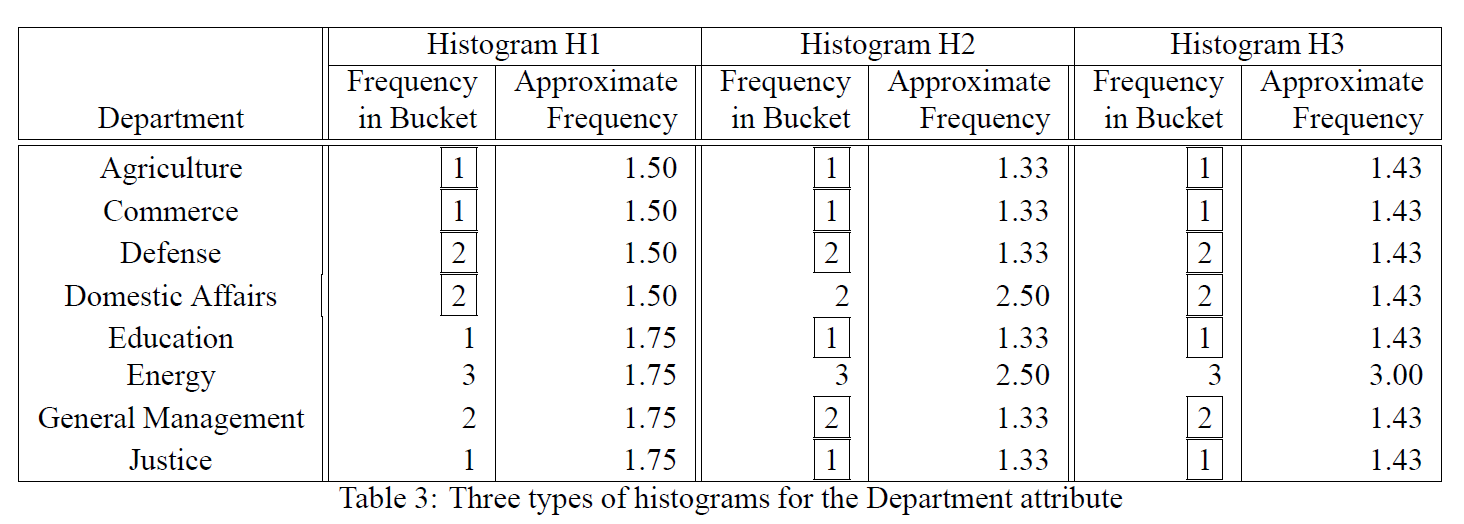
\includegraphics[width=\textwidth,height=0.79\textheight,keepaspectratio]{histogram-example-ioannidis-2.png} 
\footnote{\tiny{Изображение взято из \cite{Ioannidis1995}}}
\end{figure}
{\scriptsize
Серийная гистограмма: параметры (частоты) ассоциированные с каждым ведром больше или меньше параметров (частот) любого другого ведра. Т. е. ведра серийной гистограммы хранят вместе параметры (частоты)  близкие друг к другу и не допускают пересечение. \\~\\

H1 -- нет; H2, H3 -- да.
}
\end{frame}


%For many types of queries, an important role with respect to optimality is played by the class of serial histograms

\begin{frame}
\frametitle{Серийный класс, визуально}
\center
\begin{tikzpicture}

\filldraw[fill=blue!40!white, draw=black] (2,0.5) rectangle (8.5,2);

\filldraw[fill=blue!40!white, draw=black] (1,2.8) rectangle (4,4);

\filldraw[fill=blue!40!white, draw=black] (2.8,4.3) rectangle (3.2,4.7);

\draw[thick,->] (0,0) -- (9.5,0) node[anchor=north west] {значения};
\draw[thick,->] (0,0) -- (0,5) node[anchor=south east] {частота};

\draw[thick,-o] (1,0) -- (1,4);
\draw[thick,-o] (2,0) -- (2,2);
\draw[thick,-o] (3,0) -- (3,4.5);
\draw[thick,-o] (4,0) -- (4,3);
\draw[thick,-o] (8.5,0) -- (8.5,1);



\draw[thick,-o] (8,0) -- (8,1.5);


\end{tikzpicture}
\raggedright
Класс, серийный по частоте.

\end{frame}


\begin{frame}
\frametitle{Серийный класс}

Какие есть серийные?
\begin{itemize}
  \setlength\itemsep{1em}
  \item equi-sum (V, S) = equi-width; equi-sum (V, F) = equi-depth;
  \item v-optimal;  
  \item spline-based;
\end{itemize}

Свойства:
\begin{itemize}
  %\setlength\itemsep{1em}
  \item Доказано, что оптимальны для минимизации ошибок для определенных запросов;
  \item Дорого хранить, для оптимальности при выборках и соединениях требуют хранения в ведре всего списка значений;
  \item Часто, дополнительно приходится пользоваться индексом \cite{Ioannidis1995}.
  \begin{itemize}
    \item[] нет порядковой корелляции между значениями и частотами $\longrightarrow$ а частоту каждого атрибута считать надо! $\longrightarrow$ нужны многомерные индексы при обобщении на несколько атрибутов.
  \end{itemize}

\end{itemize}

\end{frame}


\begin{frame}
\frametitle{V-Optimal (F, F)\footnote{Наглядный пример построения: https://en.wikipedia.org/wiki/V-optimal\_histograms}}

\begin{itemize}
  \setlength\itemsep{1em}
  \item Группируют частоты, минимизируют дисперсию в ведерке;
  \item Минимизируют взвешенную дисперсию:
  $$\sum\limits_{j=1}^{\beta} n_j * V_j, $$
  где  $n_j$ количество записей в $j$ ведре, $V_j$ дисперсия \alert{частот} в $j$ ведре;
  \item Канонический алгоритм построения требует полного перебора, поэтому, пользуются эвристиками;
  \item Оптимальны для дерева с соединением по ``='', выборках и без функций.
\end{itemize}

\end{frame}

\begin{frame}
\frametitle{Spline-Based (V, C)}

\begin{figure}[htb]
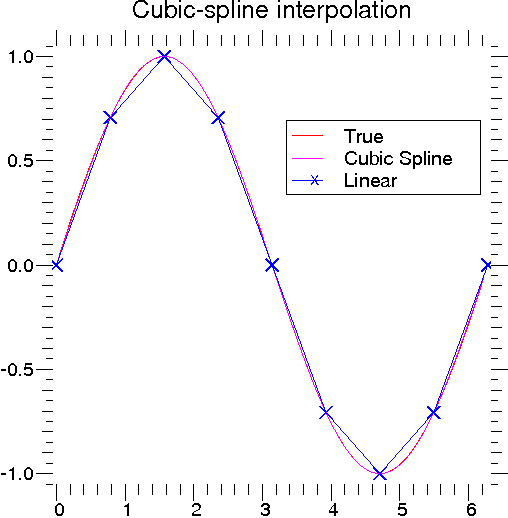
\includegraphics[width=\textwidth,height=0.39\textheight,keepaspectratio]{spline.png} 
\footnote{\tiny{Изображение взято из \url{https://www.tau.ac.il/~kineret/amit/scipy_tutorial/}}}
\end{figure}

\begin{itemize}
  \setlength\itemsep{1em}
  \item Кусочно-линейная \alert{аппроксимация} $T_{C+}$;
  \item Лучше \alert{аппроксимация} $\rightarrow$ меньше ошибка;
  \item Задача оптимальной расстановки узлов (optimal knot placement problem)~--- используют эвристический алгоритм.
\end{itemize}

\end{frame}

\begin{frame}
\frametitle{V-Optimal-End-Biased(F,F)}

\begin{itemize}
  \setlength\itemsep{1em}
  \item Класс end-biased это подкласс серийного;
  \item Идея: некоторые самые большие и некоторые самые маленькие частоты хранятся в отдельных ведрах. Остальные хранятся в одном ведре, аппроксимируются.
  \item Дешевы в построении: полный перебор за почти линейное время;
  \item Дешевы в хранении, не нужен индекс. В ведрах-синглтонах храним и значения;
  \item Подробно разобраны здесь: \cite{Ioannidis19952}.
  \end{itemize}
$\longrightarrow$ популярны в индустрии.
\end{frame}


\begin{frame}
\frametitle{Что лучше?}

\begin{figure}[htb]
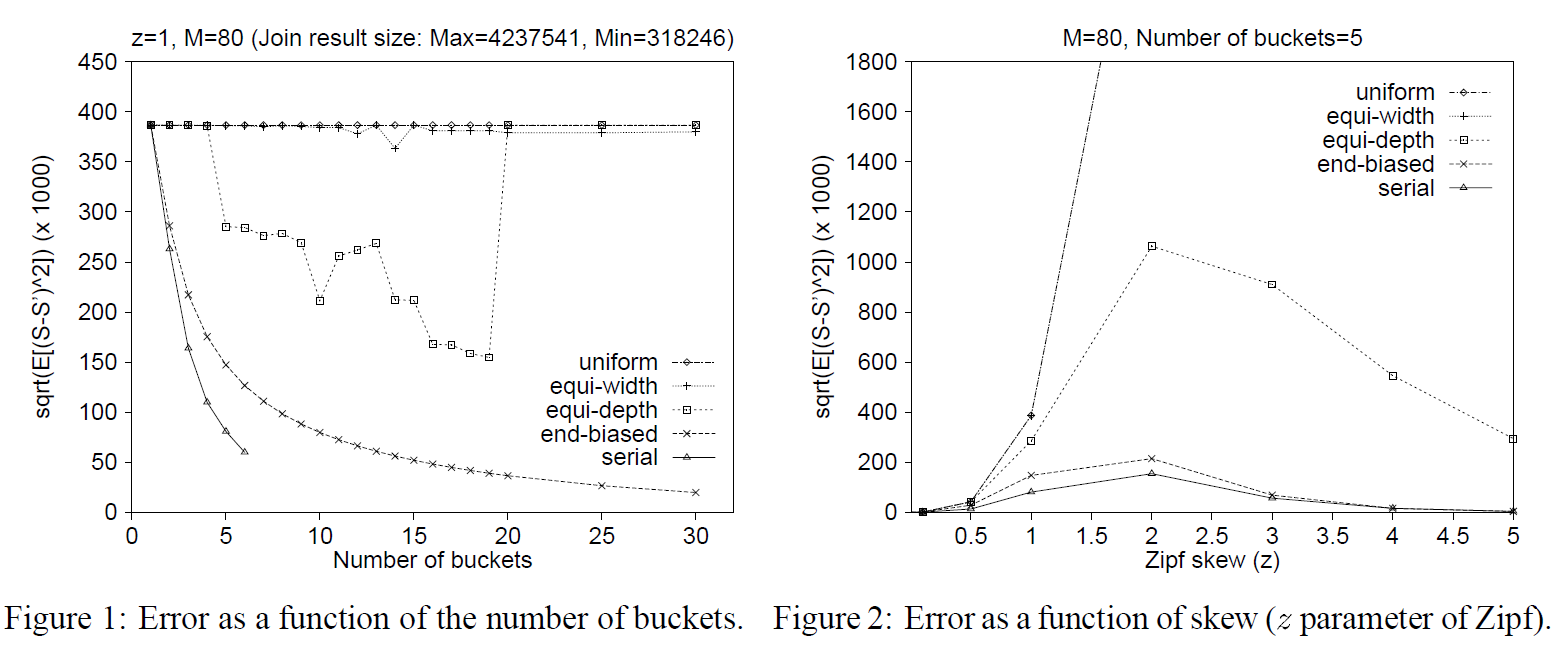
\includegraphics[width=\textwidth,height=0.65\textheight,keepaspectratio]{test.png} 
\footnote{\tiny{Изображение взято из \cite{Ioannidis1995}}}
\end{figure}

\end{frame}

\begin{frame}
\frametitle{Классификация-2}

\begin{figure}[htb]
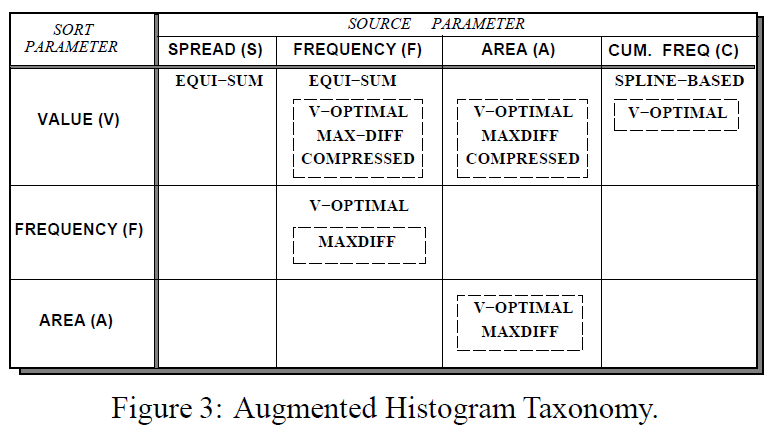
\includegraphics[width=\textwidth,height=0.65\textheight,keepaspectratio]{taxonomy-2.png} 
\footnote{\tiny{Изображение взято из \cite{Poosala1996}}}
\end{figure}

\end{frame}

\begin{frame}
\frametitle{Другие типы}
Maxdiff:
\begin{itemize}
  \item ставим границу между ведрами по двум значениям параметра-источника: если разница между ними относится к $\beta - 1$ самых больших разниц;
  \item идея: не группировать значения с сильно разными значениями параметра-источника в одно ведро;
  \item вычисляются эффективно, считаем разницу между ближайшими параметрами.
\end{itemize}

Compressed:
\begin{itemize}
  \item Самые большие значения параметра-источника хранятся отдельно в ведрах-синглтонах, остальные equi-sum;
  \item Хорошая точность при аппроксимации неравномерных распределений и/или спредов.
\end{itemize}

\end{frame}


\begin{frame}
\frametitle{Что лучше-2?}

\begin{figure}[htb]
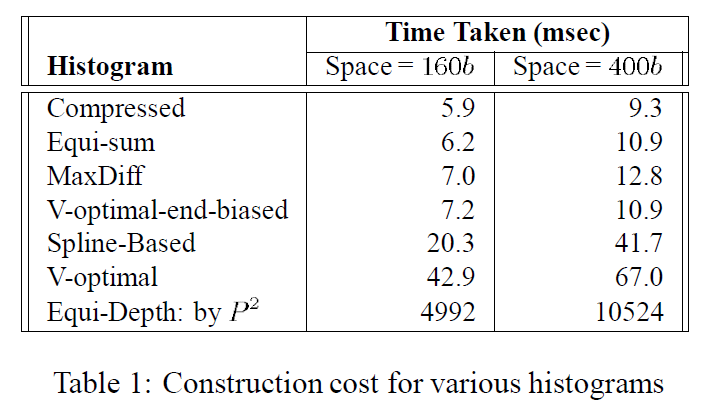
\includegraphics[width=\textwidth,height=0.65\textheight,keepaspectratio]{test-2.png} 
\footnote{\tiny{Изображение взято из \cite{Poosala1996}}}
\end{figure}

\end{frame}


\begin{frame}
\frametitle{Что лучше-3?}

\begin{figure}[htb]
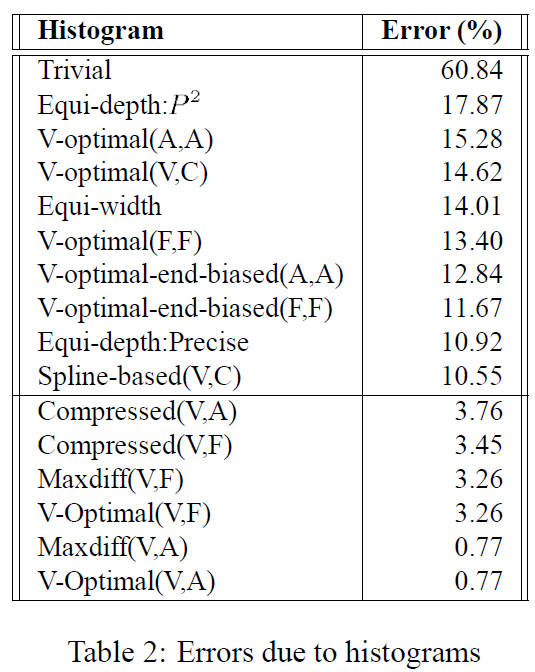
\includegraphics[width=\textwidth,height=0.80\textheight,keepaspectratio]{test-3.png} 
\footnote{\tiny{Изображение взято из \cite{Poosala1996}}}
\end{figure}

\end{frame}

\begin{frame}
	\frametitle{Альтернативы гистограммам}
	
	\begin{itemize}
		\setlength\itemsep{1em}
		\item сэмплинг~--- кажется это то, что сейчас популярно и чему сейчас гистограмный подход проигрывает;
		\item вейвлеты;
		\item нишевые методы;
		\item параметрические методы.
	\end{itemize}
	
	Гистограммы используются на практике: дешевы, могут занимать 200 \alert{байт} \cite{Ioannidis1995} и при этом быть полезными!
	
\end{frame}


\begin{frame}
	\frametitle{Оценка размера результатов: выборки}
	
	\begin{itemize}
		\setlength\itemsep{1em}
		\item Если на колонке есть ограничение типа UNIQUE, а предикат на равенство то гистограммы не нужны \smiley{};
		\item Если ограничения нет, а есть предикат $\longrightarrow$ гистограмма;
		\item Отрицание: $SEL(!p) = 1 - SEL(p)$;
		\item Если есть два предиката на одну таблицу и
		\begin{itemize}
			\item они объединены через AND то $SEL(p_1 \cup p_2) = SEL(p_1) *SEL(p_2)$
			\item они объединены через OR то $SEL(p_1 \cap p_2) = SEL(p_1) + SEL(p_2) - SEL(p_1) *SEL(p_2)$
		\end{itemize}
		Это работает если распределения \underline{независимы} то есть, атрибуты не \underline{скореллированы}.\\~\\
		Пример: пусть есть тип одежды и тип материала. Формула не сработает если оценивается селективность запроса ``шуба из меха'' (шуб не из меха не бывает!): селективность будет равна не произведению, а селективности только шубы.
		

		
	\end{itemize}
	
	
\end{frame}

\begin{frame}
	\frametitle{Оценка размера результатов: соединения}
	$R, S$~--- отношения, $|R|$~--- количество записей в $R$, $|R_A|$~--- количество уникальных значений в $R$. Тогда:

	$$ joinSize \approxeq \frac{|R| * |S|}{max(|R_A|, |S_A|)} $$
	
	Здесь A это атрибут соединения в общем случае.
	

	Как к этому пришли? Рассмотрели по-отдельности каждую запись из $R$ и прикинули сколько будет результатов в $S$. Потом наоборот.
	\\~\\
	На самом деле эта формула почти бесполезна.
	
\end{frame}

\begin{frame}
	\frametitle{Оценка размера результатов: количество уникальных значений атрибута}
	Наивно:
	\begin{itemize}
		\item Посчитать влоб: пройтись по всем данным, держать в памяти все уникальные записи и количество.
		\item Отсортировать и пройтись.
	\end{itemize}
	Недостатки серьезны $\longrightarrow$ на практике применяют HyperLogLog.\\~\\
	
	Основывается на probabilistic counting: 1.5 килобайта в памяти могут дать 2\% ошибки на $10^9+$ данных.\\~\\

	Очень хорошая демонстрация работы\footnote{http://content.research.neustar.biz/blog/hll.html}.\\~\\
	
	Есть и другие методы \cite{Harmouch2017}.\\~\\	
	
\end{frame}

\begin{frame}
	\frametitle{Что в реальности с оценками? I}
	


	\begin{figure}[htb]
		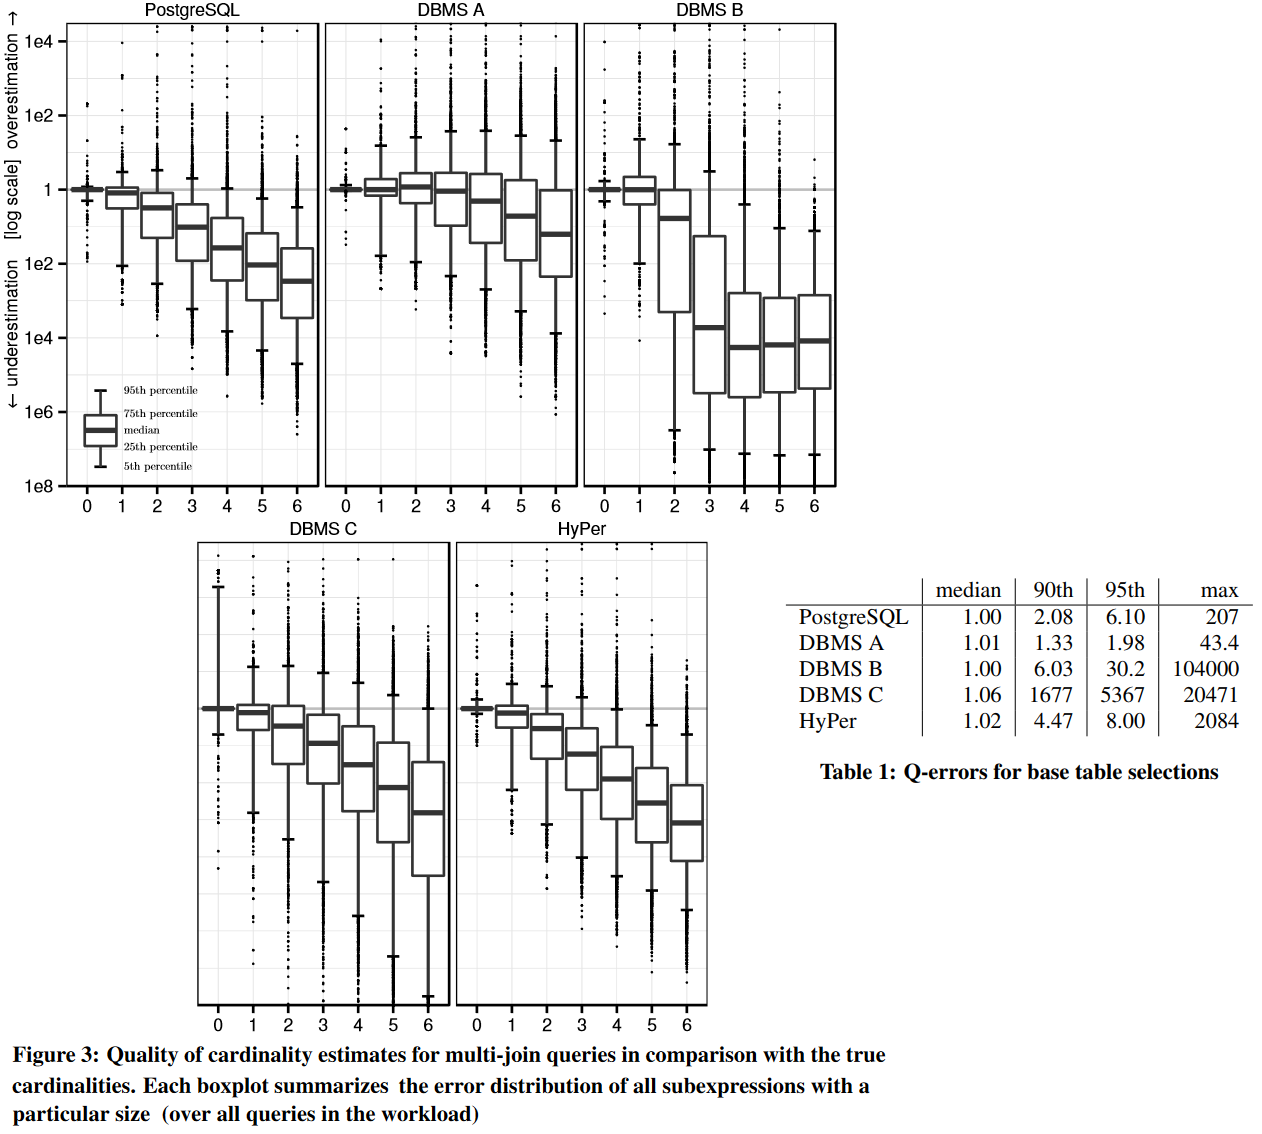
\includegraphics[width=\textwidth,height=0.80\textheight,keepaspectratio]{estimates-overall.png} 
	\end{figure}			


	
	Изображения взяты из статьи \cite{Leis2015}.
	
\end{frame}

\begin{frame}
	\frametitle{Что в реальности с оценками? II}
	\scriptsize
	Это очень важная статья. Она экспериментально показывает что модель << оценок.
	
	\begin{figure}[htb]
		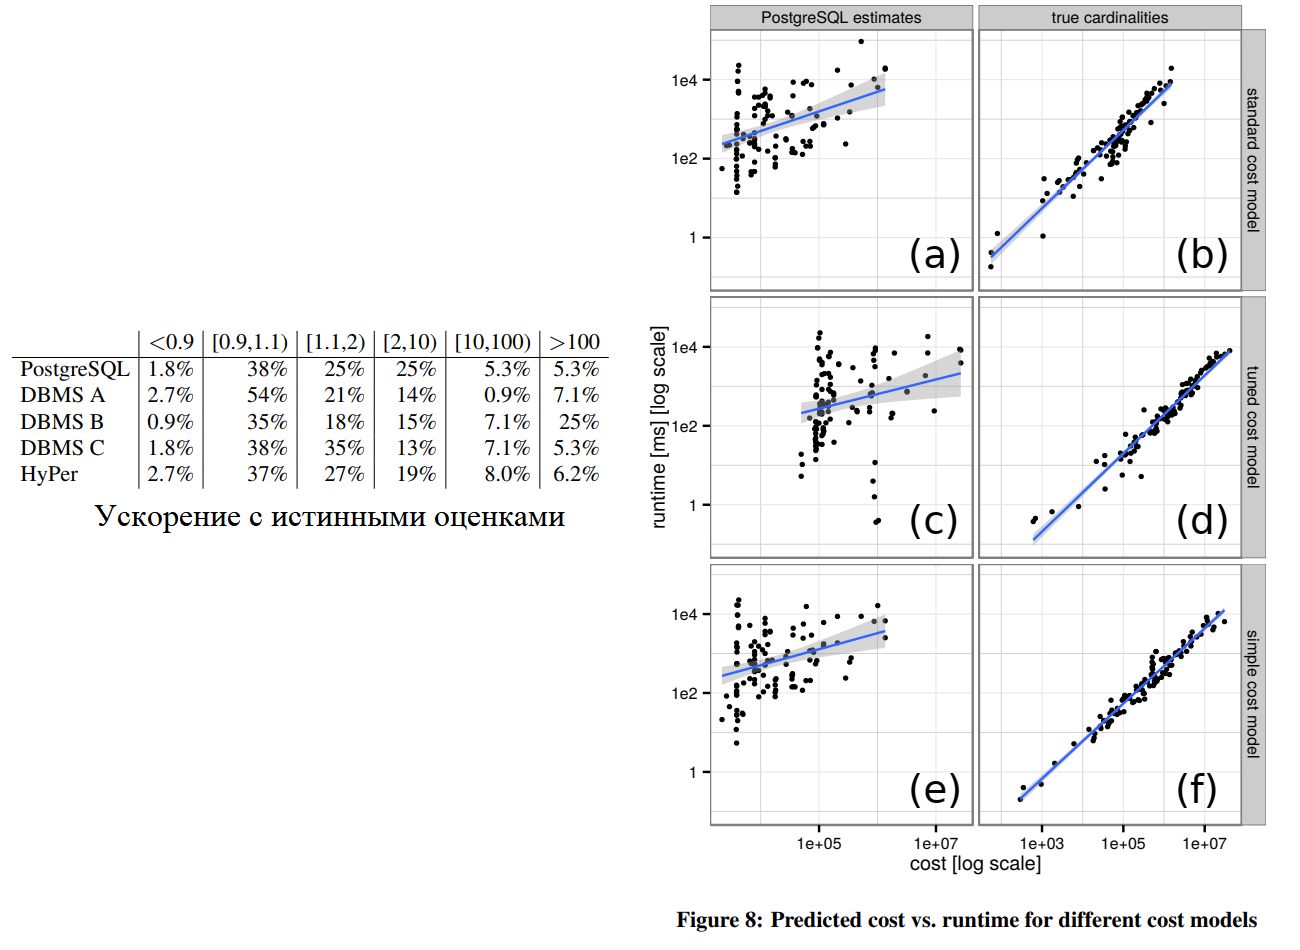
\includegraphics[width=\textwidth,height=0.70\textheight,keepaspectratio]{estimates-vs-model.png} 
	\end{figure}			
	
	
	
	Изображения взяты из статьи \cite{Leis2015}.
	
\end{frame}



\begin{frame}[allowframebreaks]
\frametitle{Ссылки}
\footnotesize{
\begin{thebibliography}{99}

\bibitem[Ioannidis, 2003] {Ioannidis2003}  Yannis Ioannidis. 2003. The history of histograms (abridged). In Proceedings of the 29th international conference on Very large data bases - Volume 29 (VLDB '03), Johann Christoph Freytag, Peter C. Lockemann, Serge Abiteboul, Michael J. Carey, Patricia G. Selinger, and Andreas Heuer (Eds.), Vol. 29. VLDB Endowment 19--30. 

\bibitem[Ioannidis and Poosala(a), 1995] {Ioannidis1995} Y. Ioannidis and V. Poosala. Histogram Based Solutions to Diverse Database Estimation Problems, IEEE Data Engineering, Vol. 18, No. 3, pp. 10--18, September 1995.

\bibitem[Poosala et al., 1996] {Poosala1996} Viswanath Poosala, Peter J. Haas, Yannis E. Ioannidis, and Eugene J. Shekita. 1996. Improved histograms for selectivity estimation of range predicates. In Proceedings of the 1996 ACM SIGMOD international conference on Management of data (SIGMOD '96), Jennifer Widom (Ed.). ACM, New York, NY, USA, 294--305. DOI=http://dx.doi.org/10.1145/233269.233342 

\bibitem[Ioannidis and Poosala(b), 1995] {Ioannidis19952}   Yannis E. Ioannidis and Viswanath Poosala. 1995. Balancing histogram optimality and practicality for query result size estimation. In Proceedings of the 1995 ACM SIGMOD international conference on Management of data (SIGMOD '95), Michael Carey and Donovan Schneider (Eds.). ACM, New York, NY, USA, 233--244. DOI=http://dx.doi.org/10.1145/223784.223841 



\bibitem[Kooi, 1980] {Kooi1980} Robert Philip Kooi. The Optimization of Queries in Relational Databases. PhD Thesis, Case Western Reserve University (1980).

\bibitem[Piatetsky-Shapiro and Connel, 1984] {Piatetsky-Shapiro1984} Gregory Piatetsky-Shapiro and Charles Connell. 1984. Accurate estimation of the number of tuples satisfying a condition. In Proceedings of the 1984 ACM SIGMOD international conference on Management of data (SIGMOD '84). ACM, New York, NY, USA, 256--276. DOI=http://dx.doi.org/10.1145/602259.602294 

\bibitem[Harmouch and Naumann, 2017] {Harmouch2017} Harmouch, H., Naumann, F.: Cardinality Estimation: An Experimental Survey.Proceedings of the VLDB Endowment (PVLDB). pp. 499--512 (2017).

\bibitem[Leis et al, 2015] {Leis2015} Viktor Leis, Andrey Gubichev, Atanas Mirchev, Peter Boncz, Alfons Kemper, and Thomas Neumann. 2015. How good are query optimizers, really? Proc. VLDB Endow. 9, 3 (November 2015), 204--215. DOI:https://doi.org/10.14778/2850583.2850594





\end{thebibliography}
}
\end{frame}


\end{document} 